\section{Het ontwerp}
\subsection{De versterker}
De AMP of versterker zorgt voor de amplificatie van het ingevoerde audio signaal. Dit wordt tot stand gebracht door het gebruik van een LM386 chip van Texas Instruments.  Ten eerste komt het audio signaal binnen bij audio-in dat in dit geval de audio jack moet voorstellen. Het audio signaal zal dan door een klein circuit heen gaan, genaamd de limiter, die ervoor zorgt dat hoge pieken in het invoersignaal gedempt worden voordat ze de LM386 bereiken. Als het signaal dan eenmaal de LM386 heeft bereikt wordt het voltage zo ongeveer met 20 vermenigvuldigd wat het minimum is van de LM386. Dit geeft ons een signaal dat op zijn hoogst de 9 volt bereikt wat gelijk staat aan de 9 volt voeding. Tussen de voeding en de chip zitten er twee capacitors die nodig zijn om de ruis zo veel mogelijk te verminderen wat weer zorgt voor een betere audio kwaliteit. Het geamplificeerde signaal is dan gereed om door de speaker afgespeeld te worden. 
\begin{figure}[ht]
    \centering
    \includegraphics[width=0.75\textwidth]{004/amp-BW}
    \caption{Versterker}
    \label{fig:Versterker}
\end{figure}

\subsection{De buffer}
Mietek
\textit{Niks ontvangen}
\begin{figure}[ht]
    \centering
    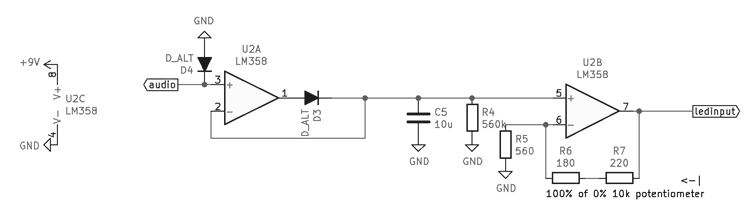
\includegraphics[width=0.75\textwidth]{004/buffer-BW}
    \caption{Buffer}
    \label{fig:Buffer}
\end{figure}

\subsection{De VU-meter}
De VU-meter geeft aan hoe hard het uitgangssignaal is dat naar de speaker gaat. Wij hebben hiervoor verscheidene metingen gedaan om op de juiste weerstanden te komen. Ons circuit werkt als volgt: wij hebben 4 comparatoren die vergelijken of het uitgangssignaal hoger is dan het aangegeven signaal, als dit zo is zal de comparator de led laten aangaan omdat de stroomkring gesloten wordt. 
\begin{figure}[ht]
    \centering
    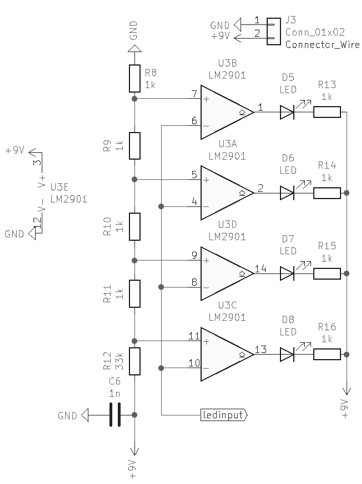
\includegraphics[angle=-90]{004/VuMeter-BW}
    \caption{VuMeter}
    \label{fig:VuMeter}
\end{figure}

\subsection{De blokdiagrammen}
Zerong
\textit{Niks ontvangen}